\documentclass[twocolumn]{article}
% \usepackage[english]{babel}
% \usepackage[T1]{fontenc}
% \usepackage{graphicx}
\usepackage{kpfonts}[maths]
\usepackage{libertine}
% \usepackage{placeins}
% \usepackage{gensymb}
\usepackage{fontspec}
\setmonofont[Mapping=tex-text]{inconsolata}
% \usepackage{subcaption}
% \usepackage{mdframed}
% \usepackage{caption}
\usepackage{amsmath}
% \usepackage{lipsum}
\usepackage{tikz}
% \usepackage{minted}
% \usepackage{lipsum}
% \usepackage{xcolor}
% \usepackage{sectsty}
\usepackage{hyperref}
% \usepackage{csquotes}
\usepackage[style=authoryear]{biblatex}
\usepackage[inline]{enumitem}


\newlist{inline-enum}{enumerate*}{1}
\setlist[inline-enum]{label=(\roman*)}

\hypersetup{
    colorlinks=true,
    urlcolor=blue,
    linkcolor=black,
    citecolor=black,
}

\definecolor{CERNblue}{HTML}{22529e}
\definecolor{CodeBg}{rgb}{0.95, 0.95, 0.95}

% \setminted{
%     % linenos=true,
%     autogobble=true,
%     frame=single,
%     % framesep=2mm,
%     % framerule=0.4pt,
%     tabsize=4,
%     fontsize=\footnotesize,
%     breaklines,
%     bgcolor=CodeBg,
% }

\usetikzlibrary{automata, positioning, arrows, shapes}
\tikzset{
  ->, % make edges directed
  >=stealth, % make the arrow heads bold
  node distance=5.5cm, % minimum distance
  every state/.style={thick, fill=gray!10, ellipse}, % properties of state nodes
  initial text=Start, % text that aappears on the start arrow
  every text node part/.style={align=center}, % allow multiline node descriptions
}

\setlist[enumerate]{itemsep=0mm}
\setlist[itemize]{itemsep=-0mm}


% \sectionfont{\color{CERNblue}}
% \subsectionfont{\color{CERNblue}}
% \subsubsectionfont{\color{CERNblue}}

\newcommand{\hypermail}[1]{\href{mailto:#1}{\texttt{<#1>}}}

\addbibresource{ref.bib}

% TODO: add a link to the repository somewhere

\title{
D7039E/E7032E\footnote{Codes of courses taken by team members at Luleå Technical University.}
--- Project: Model, Simulation and Implementation of a Mechatronical System for Use in a Mimicked Industrial Environment
}
\author{
As authored/researched/developed by:\footnote{In no particular order; All team members can be contacted via \href{mailto:vikson-6@student.ltu.se;lukkar-4@student.ltu.se;sansim-6@student.ltu.se;olemis-6@student.ltu.se;rubasp-6@student.ltu.se;alinou-6@student.ltu.se;alikhar-6@student.ltu.se}{this hyperlink}.} \\
Viktor Sonesten \hypermail{vikson-6@student.ltu.se} \\
Lukas Karlsson \hypermail{lukkar-4@student.ltu.se} \\
Simon Sandberg \hypermail{sansim-6@student.ltu.se} \\
Oleksiy Mishchenko \hypermail{olemis-6@student.ltu.se} \\
Ruben Asplund \hypermail{rubasp-6@student.ltu.se} \\
Ali Nouri \hypermail{alinou-6@student.ltu.se} \\
Ali Khademi \hypermail{alikha-6@student.ltu.se}
}
\date{\today}                   % TODO: use latest date as reported by git

\begin{document}
\maketitle

\input{sections/introduction.tex}
\section{System design and composition}
\subsection{Model}
The system is modelled in two parts: the moving base and the\ldots
% TODO: describe the moving base, and the attachment, whatever it ends up being.
% Include physical models.


% Describe the states of the system.
We argue for the folloing five states of the system:
\begin{inline-enum}
\item waiting for a command;
\item moving to a destination;
\item following a navigation-line;
\item picking an object up; and
\item dropping an object off.
\end{inline-enum}
The relation between these five states are visually described in the state machine of Fig~\ref{fig:state_machine}.
\begin{figure*}[ht]
  \centering
  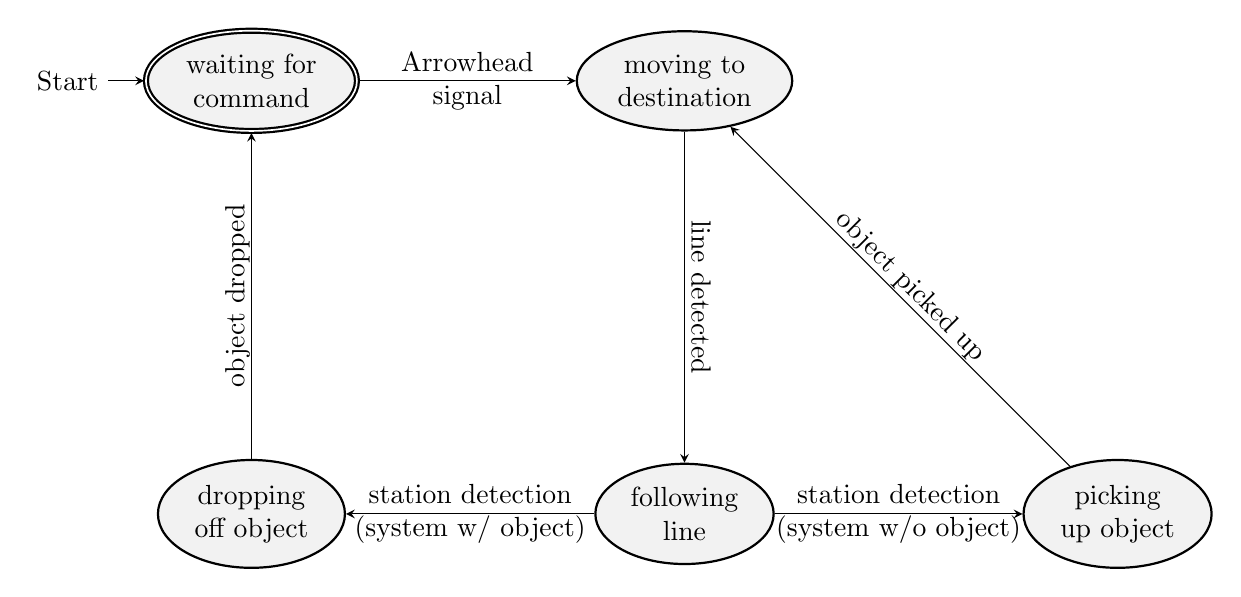
\begin{tikzpicture}
    \node[state, initial, accepting] (wait) {waiting for \\ command};
    \node[state, right of=wait] (move) {moving to \\ destination};
    \node[state, below of=move] (follow) {following \\ line};
    \node[state, right of=follow] (pickup) {picking \\ up object};
    \node[state, left of=follow] (dropoff) {dropping \\ off object};

    \path[->] (wait) edge node{Arrowhead \\ signal} (move)
    (move) edge[sloped] node{line detected \\} (follow)
    (follow) edge[sloped] node{station detection \\ (system w/o object)} (pickup)
    (follow) edge[sloped] node{station detection \\ (system w/ object)} (dropoff)
    (pickup) edge[sloped] node{object picked up \\} (move)
    (dropoff) edge[sloped] node{object dropped \\} (wait)
    ;
  \end{tikzpicture}
  \caption{High-level state machine of the system.}
  \label{fig:state_machine}
\end{figure*}
\subsubsection{Mobile platform}
The model used in this case is the unicycle model, due to the differential steering. 
This is because of the mobile platform has only two wheels/trucks and it is not able to apply any steering angle to its wheels. 
The only way this robot can change orientation is by giving different velocity on each wheel-driving servo on left- and right- side. 
With this feature it is also possible to change the orientation of the mobile platform without changing the position of the platform. 
I.e. the robot is able to spin while the right-hand sidewheels have the same velocity as the left-hand side wheels, in opposite direction. 

\begin{figure}[h!]
\centering
\includegraphics[width=0.4\textwidth]{sections/assets/car-unicycle.png}
\caption{Unicycle model of a car-like robot. 
$v_L$ and $v_R$ represent the left- and right-hand side wheels' velocities respectively. 
The robot follows a path around the instantaneous center of rotation (ICR) where $R_L$ and $R_R$ are the distances from left and right wheels to ICR respectively and $w$ is the distance between them.}
\label{fig:UnicycleModel}
\end{figure} 

As shown in Fig.~\ref{fig:UnicycleModel} The robot follows a curved path with the instantaneous center of rotation at its center. 
The left-hand side wheels have velocity $v_L$ and moves along an arc with radius $R_L$ during the time that right-hand side wheels moves along another arc with radius $R_R$ at the speed of $v_R$. 
The turning rate of the body is
        \begin{equation*}
            \dot{\theta}= \frac{v_L}{R_L} = \frac{v_R}{R_R}
        \end{equation*}
        since $R_R = R_L + W$ the expression can be simplified as
        \begin{equation}
            \dot{\theta}= \frac{v_R - v_L}{W} = \frac{v_\Delta}{W}\label{eq:ThetaDot3}
        \end{equation}
        the equations of motion for this model are
        \begin{eqnarray}
            \begin{aligned}
                \dot{x} &= v\,cos(\theta)\\
                \dot{y} &= v\,sin(\theta)\\
                \dot{\theta} &= \frac{v_\Delta}{W}
            \end{aligned}
            \label{eq:MotionEq3}
        \end{eqnarray}
        where the average velocity\parencite{Corke2011} is given by
        \begin{equation}
            v = \frac{v_R + v_L}{2} 
            \label{eq:av_velocity}
        \end{equation}{} 


\subsection{Simulation}
% Simulte the models from the previous section and show that it will work.
% Motivate regulation approach.

\subsection{Hardware}
% Explain the raspberry pi and it's attachments.

% TODO: remove this section; talk about software in `implementation.nix` instead.
\subsection{Software}

% TODO: rewrite/move elsewhere?
\subsubsection{System-external services}
The software environment generated for the Raspberry Pi automatically connects to Eduroam if credentials are available.
Eduroam places some limitations on connected clients: firewall, e.g.
To enable easy remote access to the system, a reverse SSH proxy is established with a known bastion host which has a static IP address.
By exposing this proxy via a known port on the bastion, any system connected to the Internet may trivially access the Raspberry Pi remotely via a static endpoint.
While not a necessity for the project itself, this external service is a great convenience for ad-hoc experiments and general system debugging.

% Explain the content of contrib/bastion.nix

\section{Implementation}
The git repository used throughout this project is publicly available at \href{https://github.com/tmplt/ed7039e}{Github/tmplt/ed7039e} \parencite{repo}.
If not otherwise specified, any references to a repository shall mean this repository.

% We chose to implement our System on a Raspberry Pi.
% This means our system is not in real-time (Linux too complex, other reasons)
% Allows people not versed in embedded systems to write implementations
% A proper implementation would be on a micro-controller that allows code to be run bare-metal, without having to fight with the Linux kernel.

\subsection{Milestones}
The project is divided into four milestones:
\begin{enumerate}
\item \textbf{Two-dimensional navigation:}
  the system should be able to determine its coordinates in a ad-hoc, local grid.
  From its initial position, it should then be able to respond to movement commands on the form ``move to position $(x, y)$''.

\item \textbf{Navigation-line detection:}
  using the subsystem for two-dimensional navigation, the system is to cross a line on the floor,
  thus detecting it and follow it towards the station.

\item \textbf{Station proximity detection, object pickup:}
  once the navigation-line is being followed, the system is to sense when it is sufficiently close to the station to readily use its arm to pick the object up.

\item \textbf{Object displacement, drop-off:}
  after the object has been picked up, the system is to move to another station, find its navigation-line, follow it, and drop the object.
  Note that this milestone is a permutation of the combination of the previous milestones: the same phases should be done in the same order,
  but the system is to move to the second station instead and execute the pickup-process in reverse.
\end{enumerate}

% TODO: write here when each milestone was reached and why it took the time it did

\subsection{Prototyping}
% Here we describe the prototyping stages of the system's components if anything
% out of the ordinary pops up.

\subsubsection{NixOS}
% Introduce NixOS and what is gives us
In this project we have chosen to use NixOS as the operating system on which to run our software.
NixOS is a Linux distibutiton (henceforth referred to as a ``distro'') based upon the Nix package manager (and the terms will be used interchangibly henceforth) that aims to be
\begin{inline-enum}
\item reproducible:
  ``packages [are built] in isolation from each other. [\ldots] they are reproducible and don't have any undeclared dependencies.''\footnote{A positive side-effect of this feature is the complete mitigation of ``dependency hell'': a term relating to a set of problems that commonly arise if multiple versions of a dependency are installed on a system.};
  so if a package works on one machine, it will work on any machine.
  Also, when building a package on multiple machine, all machines will yield the exact same output file tree.
\item Declarative:
  packages are described in expressions that are trivially shared and combined with other package declarations; and
\item reliable:
  ``installing or upgrading one package cannot break other packages''.
\end{inline-enum}~\parencite{nixos.org}

Effectively, NixOS allows us to functionally declare our system in a single (or multiple) expressions ---
that is: Nix enables us to describe the software components of our system in a common manner and how they relate to eachother.
The realization of these expressions can be seen in the repository's \texttt{*.nix} files.
Of particular interest is \texttt{mmc-image.nix}: evaluating this expression generates a bootable image readily flashed onto a MultiMediaCard (MMC)\footnote{Commonly referred to as: SD card, memory card.} that contains the full softare stack and operation instuctions of our robot system.
With the combination of git we can thus version control not only our custom software, but all its dependencies and the complete system behavior.

% How does it differ from a conventional disto?
NixOS is a contrast to the conventional Linux distribution where changes are made to the system via iterative global changes to the system state:
the installation and configuration of software piece-by-piece, for example.
In this mode, it is common to apply ``small changes'' that eventually coalesce into a significant diversion from the originally intended system behavior ---
changes made are not always documented which create a dependency on the ever-changing global state of the system (that is, the file system in which the system is prototyped/implemented).
Of note within this mode is that if the file sysetm is lost, many hours of work may have been wasted if necessary precautions weren't adhered to (by all project members) from the start of the project (such as writing a script that apply all global state changes from a fresh install, for example).
Our usage of NixOS \textit{forces} us to adhere to such precautions.

% What are the negatives of NixOS?
NixOS is no silver bullet, however.
Because of its design, whenever something is to be implemented on NixOS it must be done properly the first time.
Its non-adherence to the Filesystem Hierarchy Standard (FHS)\footnote{the existance and FHS-defined usage of \texttt{/usr}, \texttt{/lib}, \texttt{/var}, and other system directories.} breaks both the build and execution process of many programs.
Unless a program is portably written, it must be patched before it can be used on NixOS where all system files exist under \texttt{/nix/store} which is required to enable the features enumerated in the previous paragraphs.

% Hardware issues
Another problem is the distro's relative infancy to other distros, particularly when it comes to hardware support.
NixOS ships with a generic Linux kernel.
A generic kernel is expected to run on a generic system.
Because of the availability of hardware peripherals such as general-purpose input/output pins, GPIO;
universal asynchronous receiver-transmitter, UART;
serial peripheral interface, SPI; and other on the Raspberry Pi we use in this project, our system is not generic.
The result of this is that these peripherals, which we all need, simply do not work.
Fortunately, some work has already been done (and is still being done) by the NixOS community to remedy this.
By applying a so called device-tree overlay on the Linux kernel (and thus describing how an otherwise unknown peripheral may be utilized) SPI was successfully enabled,
which was required to actuate our robot's motors.
Other components we required could be utilized by help of the Raspberry Pi's USB port (fortunately a generic peripheral).
Had we instead opted to use a distro officially supposted by the Raspberry Pi, all of these peripherals would simply work out of the box, but we would then loose the featuses enumerated above.

% TODO: what problems does NixOS cause?
% * We cannot use vscode-remote
% * We cannot nix-shell into a shell with ALL appropriate python libs (whatever + brickpi3) because the new env prepends the build one in PATH.
% ...

\subsubsection{Decawave}
This project uses Decawave (or more specifically: a DWM1001 development board) for two-dimensional positioning.
The development board constitutes of the ultra wide-band module itself, the DWM1001C, an accelerometer,
and a Raspberry Pi-compatible GPIO-header.
Via communication over UART, we are able to query its measured position as reported by help of the Decawave anchor nodes\footnote{An anchor is another development board configured for static installation at a known coordinate, used for position calculation. A non-static device with unknown coordinates (as is used in our system) is known as a tag.},
and use this data to figure out where our system is located in the mimicked factory.

% Describe the TLV API we wanted to use.
The device (henceforth referred to as a/the ``DWM'') exposes two modes over UART which we can use to extract data of interest.
One of the modes is a type-length-value (TLV) API which is very suitable for automated interaction:
to extract data using this mode, we need only write three bytes on the form \texttt{\textbf{MSB}}, \texttt{\textbf{MSB-1}}, \texttt{\textbf{MSB-2}}, \texttt{\textbf{...}} where:
\begin{description}
\item[\texttt{MSB}] is the \textit{type} of data we want to send. We specify \texttt{0x40} to call a function via the API.
\item[\texttt{MSB-1}] is the value \textit{value} we want to sent. We specify (for example) \texttt{0x02} to call a function asking for the DWM position.
\item[\texttt{MSB-2}] is the length of the data we want to send. Function \texttt{0x02} takes no payload, so we specifify \texttt{0x00} here.
\item[\texttt{...}] would be a payload of length \texttt{\textbf{MSB-2}} had the function type taken a payload of non-zero size.
\end{description}
One sequece of these bytes constitute a TLV ``frame''.

% Explain the TLV frames, and how nice they are to work with.
After this frame has been written over the serial connection we receive two TLV frames in response:
the first will denote whether the function call was successful (three bytes) and the second the function return data (at least three bytes).
If the first frame says success, we read the next two bytes from which we will know what kind of data the remaining incoming bytes should be interpreted as,
and how much more we should read.
Implementation-wise, always knowing how much data to read allows for performant I/O\footnote{input/output operations: many of which require calling system functions; this is a relatively costly operation.} and easier error handling.
It also allows easy construction of the LCM messages, because they are just a single \texttt{memcpy(3)}\footnote{\texttt{memcpy} - copy memory area: a common operation where a given amount of bytes are copied from a source adress to a destination adress.} away as the byte stream can be trivially represented as a \texttt{struct} following the API documentation.

% No access to acceleration data using the TLV API; generic shell required.
Unfortunately, the TLV API does not expose a function for reading the accelerometer data which we require do estimate the direction of our robot.
A command is, however, readibly available via the interactive shell mode.
This mode instead replies in a human-readable format, but without telling us how many bytes are to be read, and in what way to interpret the data we read.
Fortunately, when the shell is ready to process new input, it writes a ``\texttt{dwm>}'' shell prompt;
we simply read the response until this string is encountered.
This ultimately require us to perform more I/O operations and parse the data upon reception, an operation that is slower than a mere \texttt{memcpy},
but is nevertheless readibly available via a proper call to the \texttt{scanf(3)} family of functions.

An alternative approach where both the TLV API and the shell mode was used was tested but ultimately scrapped:
the time to transition from the TLV API to the shell mode took approximately $1$~s, which broke our $10$~Hz requirement.

\textit{Why} accelerometer data can be queried in one mode but not the other is presently unknown.
We surmise that the existance of the shell mode is for debugging purposes only (because of its human readable format --- and its insistance of using different methods of formatting for similar data types) and that accelerometer data is omitted from the TLV API because it is used by the internal localization functions to detect when the hardware is stationary, or because the developers simply did not foresee this kind of utilization, or both.

Nevertheless, the data we receive when asking for the position is a tuple of
$(x, y, z, q)$, where
\begin{description}
\item[$(x, y, z)$] is the reported coordinate in millimeters in three-dimensional space, and
\item[$q$] is the quality factor: a measure of how sure the device is of the coordinates.
\end{description}

Of note is that the decive cannot approximate its position unless it can connect to at least three anchors.
Additionally, the quality factor, $q$, is higher when connected to four anchors.
During measurements, and if there are more than four anchors available, it will chose the best four anchors to calculate its position. % What does "best" mean here? Refer to documentation.
Because of this, we will then have to consider that our system may suddenly no longer be able fo find its position,
and decide what should be done in order to establish a connection with the disconnected anchors.

Additionally, the data we receive when asking for the acceleration is a tuple of $(x, y, z)$, where
\begin{description}
\item[$(x, y, z)$] is the reported acceleration in three-dimensional space.
\end{description}
% TODO: explain how the register values are calculated to m/s^2

% The data can be considered a random process.

% (X, Y, Z, Q); how is Q calculated?
% What should we do if we cannot connect to 4 anchors at once, a wait?
% Mention that:
% - we have to account for the fact when we tag cannot connect to at least 3 anchors.
% - Qualitative data depends a lot on the positioning of the anchors
% - Built-in 3-axis accelerometer
% - Raspberry Pi compatible GPIO header. Communication via UART.
% - How should we interpset data? It is random proccess? Can we consider noise gaussian?

% TODO:
% RPi UART problems

\subsubsection{BrickPi3}
The BrickPi3 is a peripheral that allows a Raspberry Pi to work with LEGO Mindstorms hardware.
It works by communicating via the SPI function pins of the Raspberry Pi.
The recommended way to install all necessary components is via a \texttt{curl -k | bash}.
There are a few issues with this approach:
\begin{inline-enum}
\item \texttt{-k} is an alias for \texttt{--insecure};
  the recommended approach is thus to not verify the server certificate ---
  this allows a bad actor to feed you malicious code if they have access to your DNS or the target domain.
\item A \texttt{curl | bash} is bad practise for installation purposes as it commonly installs files that are disconnected from the system's package manager.
\item A \texttt{curl | bash} can be detected server-side and thus can conditionally feed a user malicious code.
  A dowload of the code first may thus pass a manual inspection before execution. \parencite{curl-bash}
\end{inline-enum}

Because we use NixOS, the content of the script had to be inspected so that an equivalent Nix expression could be written ---
see \texttt{nix/brickpi3.nix} for the final result.
Upon inspection, a few oddities stood out. The script:
\begin{enumerate}
\item expects and requires the script to be run by the user \texttt{pi}\footnote{Not all users of the peripheral is \texttt{pi}. For example, we use it as \texttt{root} while prototyping.};
\item changes the ownership of a directory with \texttt{sudo(8)} on files under \texttt{/home/pi}, to \texttt{pi}\footnote{In this context, the operations could all have been done as \texttt{pi}.};
\item insecurely downloads multiple scripts and executes them silently --- the downloaded scrips do the same;
\item configures an \texttt{apt(8)} repository (and thus requires to be run on a Debian derivative) for \texttt{npm(1)},
  the Node JavaScript package manager, but never installs or executes any JavaScript packages;
\item installs a C++ source file under \texttt{/usr/local/include}\footnote{A proper installation would be to build a shared library which can then be dynamically linked to when using the C++ drivers.};
\item downloads a precompiled version of \texttt{openocd(1)}, a on-chip debugger and programmer,
  and copies the files into system directories\footnote{No changes are made to the software, according to the mirror's documentation. An installation should instead then be made with the package manager, which is otherwise used in the scripts to install other components}, and then never uses it;
\item runs \texttt{git(1)} as a privileged user, sometimes.
\end{enumerate}
The above list is truncated for sake of brevity.

After a thorough manual inspection of all scripts it was found that only a single Python library (with a single dependency) had to be installed.
The final Nix expression is thus a combination of two \texttt{python3Packages.buildPythonPackage} where both sources are securely downloaded from official mirrors and verified with a known checksum.
We conclude that the usage of this Nix expression leaves the system in a proper state (which the official installation script does not, by oddity 5 and 6\footnote{we consider a proper state of system one in which all installed software components are tracked by the package manager(s).}) and greatly decreases the number of attack vectors with which to run malicious code on our system.

% What need to be done to be able to stack BrickPi3s?

\subsubsection{RobotOS}
% We wanted to use ROS as it was very common to the problem space, and had a lot of readily available solutions for common robot problems.
It was initially decided that the robot system would be implemented with RobotOS (ROS), ``a set of software libraries and tools that help you build robot applications.''\footnote{See \href{https://www.ros.org/}{https://www.ros.org/}.}
The chief reason was its common application in the problem space, its API for communicating different types of messages between different programs\footnote{Known as inter-process communication (IPC).} (in this context known as ``nodes''), and the many readily available solutions to problems we were likely to stumble upon.
% Only officially supports very specific Ubuntu versions, and while probably very applicable to use Nix in this case, it was deemed
% composing ROS on Nix would take too long. (the dependency tree is HUGE)
However, ROS is only officially supported on very specific versions of Ubuntu (at this time of writing), a disto we were not using and a disto that had a very different design philosophies from NixOS;
using ROS on NixOS would thus require a Nix expression to be written that correctly packages the software.
At this point, it was surmised that ROS made several assumption about the global system state that had to be adressed during packaging.
This reason alone would likely require a lot of prototyping time for a simple proof-of-concept execution.
A consultation from another effort to port ROS to an unofficial repository showed that a full desktop installation is constituted of up to 460 packages.\footnote{See \href{https://github.com/ros-noetic-arch}{https://github.com/ros-noetic-arch}, which packages RobotOS to Arch Linux, a distro that is not officially supported by the RobotOS project. Each repository corresponds to a ROS package.}
It was thus decided to find an alternative to RobotOS due to time constrains.

\subsubsection{LCM}
% Trivial to package: just a simple mkDerivation. Nodes are similarly easily packaged. See `nix/software-nodes.nix`.
Lightweight Communications and Marshalling (LCM) ``is a set of libraries and tools for message passing and data marshalling [\ldots] It provides a publish/subscribe message passing model and automatic marshalling/unmarshalling code generation with bindings for applications''.
LCM effectively provides a set of simple functions that enable IPC with the benefit of not requiring a special-purpose daemon (as is required when running ROS).
In difference to ROS, LCM supports any GNU/Linux system (and thus NixOS) and relies on UDP multicasting for broadcasting purposes.
Its short list of dependencies made LCM trivial to package to NixOS: the final expression in \texttt{nix/software-nodes.nix} can be summarized as a \texttt{stdenv.mkDerivation} and the whitelisting of an UDP port in the system firewall.

% Support for C and Python which we have decided to use thus far.
% The core component of ROS we wanted was the message-passing (IPC) component, which this library provides for ANY POSIX-compliant system.
Thus, as LCM:
\begin{inline-enum}
\item enables us to trivially utilize IPC with different message types;
\item has bindings for C and Python; and
\item is trivially packaged,
\end{inline-enum}
it was decided that our robot system would be implemented with help of it in place of ROS.

\input{sections/results.tex}
\input{sections/conclusion.tex}
\section{Future improvements}
% Talk about how an embedded system would be more suitable for this project:
% * compass IC
% * interrupts
% * no complications with Rich OSs (Linux)
%
% Also talk somewhere about why we didnt design an embedded system to begin with.

\appendix
\section{Team members}
The team's members are below listed (in no particular order) along with their areas of concern throughout the development of this project.
Emails are available on the title page of this document.

\begin{description}
\item[Viktor Sonesten] Repository maintainership; software packaging via
  Nix; embedded data acquisition from the Decawave hardware; report
  typesetting; LCM support; team lead; authorship of sections
  §\ref{intro-background}--§\ref{intro-limits}, introduction of
  §\ref{sec:sys-design}, §\ref{sec:impl}--§\ref{sec:LCM},
  §\ref{sec:nodes}, §\ref{sec:improvements},
  appendix~\ref{sec:workflow}.

    \item[Lukas Karlsson]
    Embedded programming and
    Computer vision/position control.

    \item[Simon Sandberg]
    Hardware of robot, robot arm motion control;
    Forward and inverse kinematics of robot arm;
    Robot arm controller design;
    and embedded programming for robot motion; report
    typesetting; authorship of sections §\ref{sec:simon1}, §\ref{sec:simon2}, §\ref{sec:simon3}, §\ref{sec:simon4}, §\ref{sec:simon5}, §\ref{sec:simon6};
    §\ref{sec:simon19}, §\ref{sec:simon7}, §\ref{sec:simon8}, §\ref{sec:simon9}, §\ref{sec:simon10}, §\ref{sec:simon11}, §\ref{sec:simon12}, §\ref{sec:simon13};
    §\ref{sec:simon14}, §\ref{sec:simon15}, §\ref{sec:simon16}, §\ref{sec:simon17}, §\ref{sec:simon18};
    sections about controllers and tuning of controllers in results section, part of robot arm/hardware/controllers in improvements;
    part about robot arm/controllers of arm in conclusion.

    \item[Oleksiy Mishchenko]
    Design and implementation of line following navigations system;
    Hardware of robot, and embedded programming for mobile platform motion; report
    typesetting; authorship of sections §3.4.1, §3.4.2, §3.5, §3.5.1, §3.5.2, §3.5.3, §3.7.5, 4.3.1, 4.3.2, 4.3.3, 4.3.4;
   

    \item[Ruben Asplund]
    Arrowhead integration and embedded programming.
    Authorship of sections §\ref{sec:ruben1}, §\ref{sec:ruben2} and the Arrowhead node in §\ref{sec:nodes}.

    \item[Ali Nouri]
    Modeling, simulation and implementation of the mobile platform;
    Control and navigation system design;
    Authorship of sections §2.1.1, §2.2.1, §3.3.

    \item[Ali Khademi]
    Dynamic equations and controller design for position.
\end{description}

\input{sections/workflow.tex}

% \section{System composition}
% The current plan is to build the robot mostly with the lego ev3 parts.\\ The mobile platform will be built with the parts present in the package given to the group in the beginning of the project. The arm, which will grip the cube, will be built from external lego parts and motors, the list of these parts will be submitted furing this Tuesday. A resberry pie will be used for the communication between sensors and motors, all calculations for the control systems will also be computed int it. A preliminary model has been calculated for the forward kinematics of the system, this will probably be updated and an inverse kinematic model will be derived. The decision has not yet been made on how the location of the robot will be calculatedl, some of the possible navigation systems that have been discussed are; LIDAR, using deckawave together with a sonar, using wifi triangulation and other solutions. 

\subsection{Structure of work}
\subsubsection{Milestones}
\subsubsection{Tecchnical solutions in the project}

\printbibliography

\end{document}
